\section{Results}

\begin{raggedright}
\subsection{The evolution of adaptive phenotypic plasticity slows evolutionary change in fluctuating environments}
\end{raggedright}

%%%%%%%%%%%%%%%%%%%%%%%%%%%%%%%%%
% Results to report (2021-02-08 experiment)
% ----- GENERATIONS -----
% - average generations elapsed (of a population)
%   - NON-PLASTIC (median: 41768.65) > PLASTIC (median: 31697.65) > STATIC (median: 30839.75)
%   condition     mean    sd
%   <chr>        <dbl> <dbl>
% 1 NON-PLASTIC 41090. 2702.
% 2 PLASTIC     31016. 2615.
% 3 STATIC      30002. 3011.

% 
% ----- SWEEPS -----
% - coalescence events (total)
%   - NON-PLASTIC (median: 663.5) > ( PLASTIC (median: 45.5) ~~ STATIC (median: 45) )
% - Average number of generations between coalescence events (gens / sweeps)
%   - ( PLASTIC (median: 685.001780758557) ~~ STATIC (median: 693.676265008576) ) > NON-PLASTIC (median: 62.0184902295191) 
% 
% ----- PHENOTYPIC VOLATILITY -----
% - phenotypic volatility (total)
%   - i.e., total number of times phenotypes change along lineages
%   - NON-PLASTIC (median: 1868) > PLASTIC (median: 2) > STATIC (median: 0)
% - phenotypic volatility / lineage length
%   - i.e., how often do genomic changes reflect changes in phenotype? 
%   - NON-PLASTIC (median: 0.437) > PLASTIC (median: 0.0022) > STATIC (median: 0)
% - phenotypic volatility / generations
%   - i.e., per-offspring rate of phenotypic changes
%   - NON-PLASTIC (median: 0.0447) > PLASTIC (median: 6.33e-05) > STATIC (median: 0)
% 
% ----- MUTATION ACCUMULATION -----
% - mutation accumulation (total)
%   - NON-PLASTIC (median: 4657.5) > STATIC (median: 1100) > PLASTIC (median: 998.5)
% - mutation accumulation / lineage length
%   - NON-PLASTIC (median: 1.10048311715591) > STATIC (median: 1.03794597464116) > PLASTIC (median: 1.0328599144651) 
% - mutation accumulation / generation
%   - NON-PLASTIC (median: 0.11) > STATIC (median: 0.0368) > PLASTIC (median: 0.0319) 
% 
% ----- MUTATIONAL EFFECTS -----
% - fraction of mutational steps that alter (aggregate) phenotype
%   - NON-PLASTIC (mean: 0.434007, CI [0.4242,  0.4406]) > PLASTIC (mean: 0.002717008, 0.0020,  0.0035) > STATIC (mean: 0.0006788834, CI [0.0004,  0.0009])
% - fraction of phenotype-altering mutation steps that alter unexpressed phenotype (PLASTIC condition only)
%   - mean: 0.8247126 CI [0.7443,  0.8994]
% - fraction of mutations that affect unexpressed phenotype that are deleterious (PLASTIC only)
%   - mean: 0.5172414 CI [0.4402,  0.5977]
% - fraction of mutations that affect unexpressed phenotype that are beneficial (PLASTIC only)
%   - mean: 0.4827586 CI [0.4046,  0.5598]
%%%%%%%%%%%%%%%%%%%%%%%%%%%%%%%%%


\begin{figure}[ht!]
    \centering
    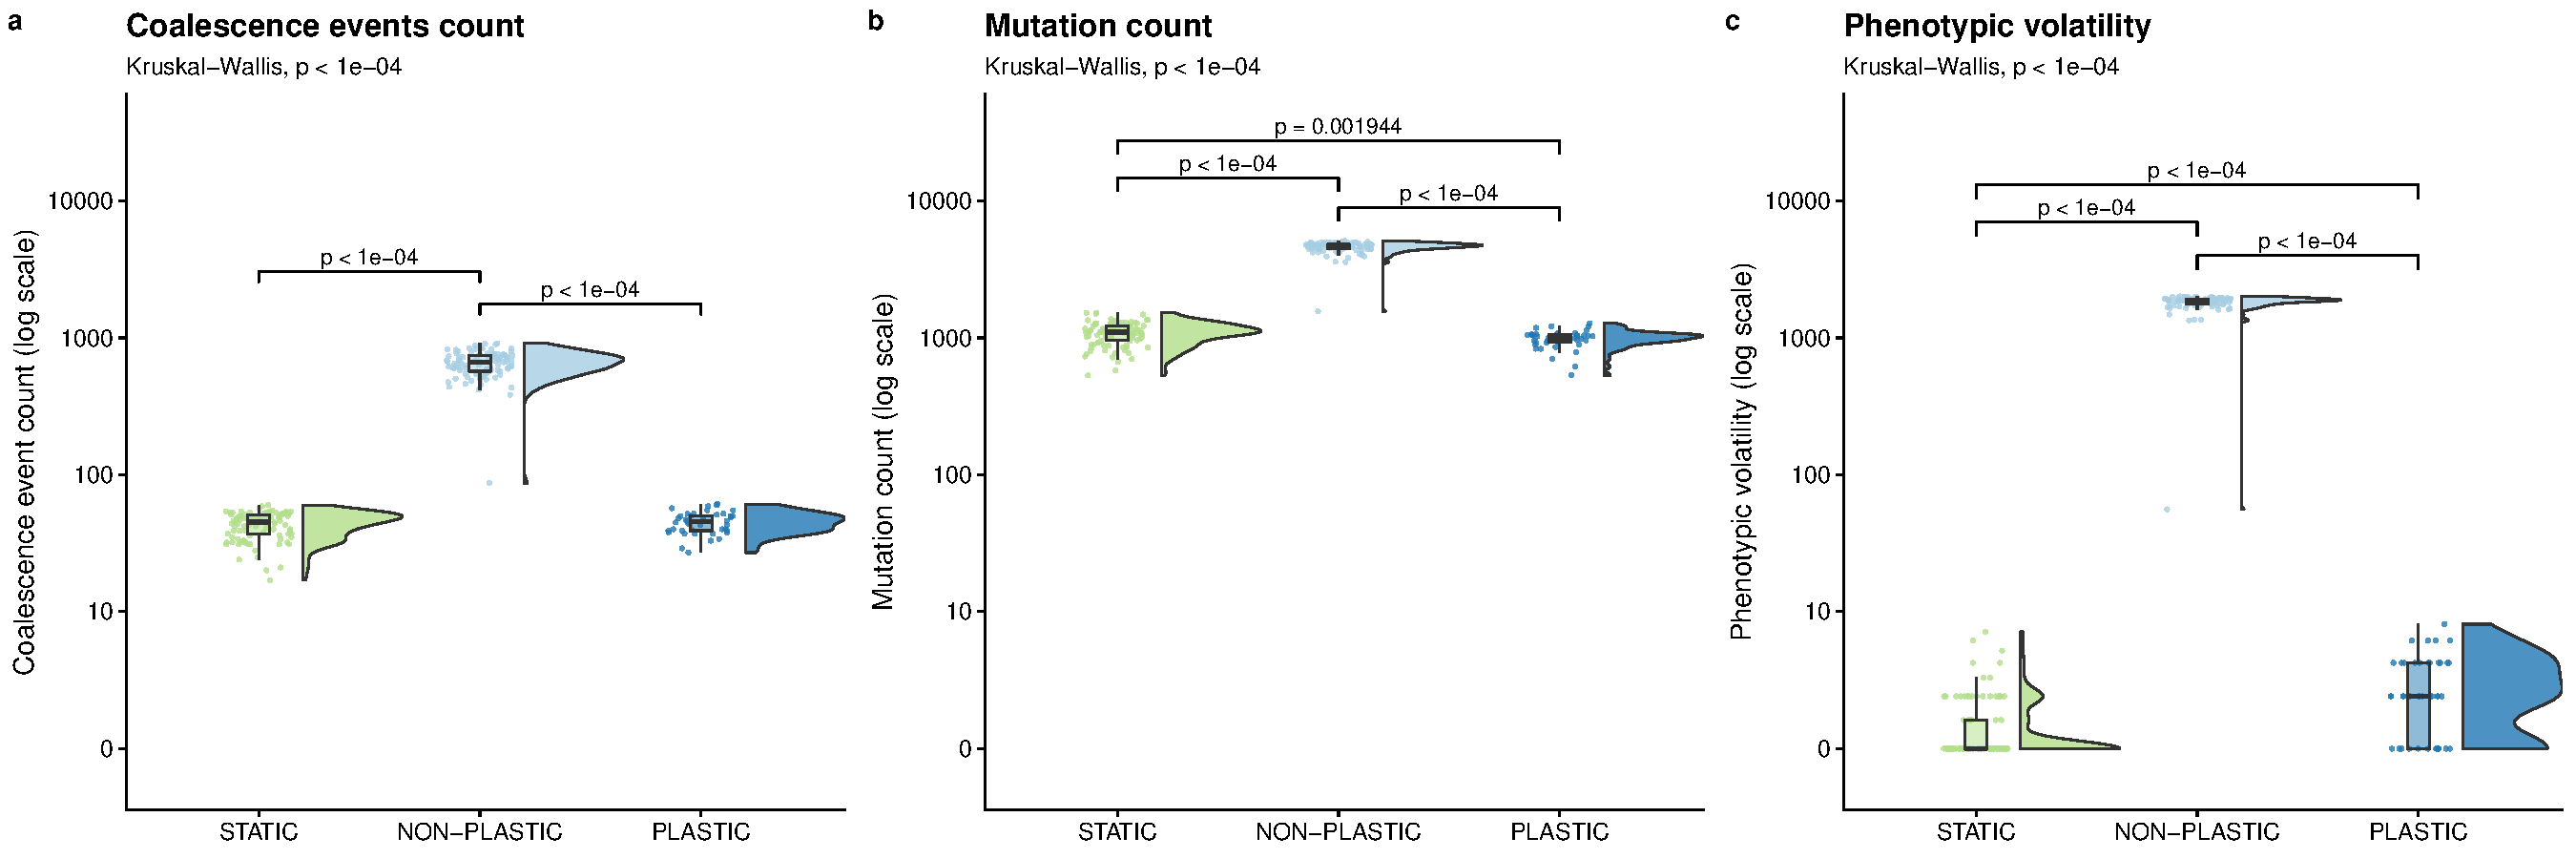
\includegraphics[width=1\textwidth]{chapters/03-evolutionary-consequences-of-plasticity/media/evolutionary-change-magnitude-panel.pdf}
    \caption{\small
    \textbf{Magnitude of evolutionary change.}
    Raincloud plots \citep{allen_raincloud_2019} of 
    (a) coalescence event count, 
    (b) mutation count, 
    and (c) phenotypic volatility. 
    See Table \ref{chapter:consequences-of-plasticity:tab:metrics-definitions} for descriptions of each metric.
    Each plot is annotated with statistically significant comparisons (Bonferroni-corrected pairwise Wilcoxon rank-sum tests).
    Note that adaptive phenotypic plasticity evolved in \evolutionaryChangeRatePlasticReps\ of \evolutionaryChangeRateReplicates\ replicates from the PLASTIC treatment during phase one of this experiment; we used this more limited group to found \evolutionaryChangeRatePlasticReps\ phase-two PLASTIC replicates from which we report these PLASTIC data.
    }
    \label{chapter:consequences-of-plasticity:fig:evolutionary-dynamics-magnitude}
\end{figure}

% -- Magnitude of evolutionary change --
In experimental \hyperref[chapter:consequences-of-plasticity:sec:methods:experiment:evolutionary-change-rate]{phase 2A},
we tested whether the evolution of adaptive phenotypic plasticity constrained or promoted subsequent evolutionary change in a fluctuating environment. 
First, we compared the total amount of evolutionary change in populations evolved under the PLASTIC, NON-PLASTIC, and STATIC treatments as measured by coalescence event count, mutation count, and phenotypic volatility (Figure \ref{chapter:consequences-of-plasticity:fig:evolutionary-dynamics-magnitude}).
According to each of these metrics, NON-PLASTIC populations experienced a larger magnitude of evolutionary change than either PLASTIC or STATIC populations.
We observed significantly higher coalescence event counts in NON-PLASTIC populations than in PLASTIC or STATIC populations (Figure \ref{chapter:consequences-of-plasticity:fig:evolutionary-dynamics-magnitude}a).
NON-PLASTIC lineages had significantly higher mutation counts (Figure \ref{chapter:consequences-of-plasticity:fig:evolutionary-dynamics-magnitude}b) and phenotypic volatility than PLASTIC or STATIC lineages (Figure \ref{chapter:consequences-of-plasticity:fig:evolutionary-dynamics-magnitude}c).

% -- Elapsed generations --
Changing environments have been shown to increase generational turnover in Avida populations \citep{canino-koning_evolution_2016}, which could explain why we observe a larger magnitude of evolutionary change at the end of 200,000 updates of evolution in NON-PLASTIC populations. 
Indeed, we found that significantly more generations of evolution elapsed in NON-PLASTIC populations (mean of $41090\pm2702$ std. dev.) than in PLASTIC (mean of $31016\pm2615$ std. dev.) or STATIC (mean of $30002\pm3011$ std. dev.) populations during phase 2A (corrected Wilcoxon rank-sum tests, p $<10^{-4}$).

% -- Rate of evolutionary change => intuition --
To evaluate whether increased generational turnover explains the greater magnitude of evolutionary change in NON-PLASTIC populations, we examined the average number of generations between coalescence events and the mutational stability of lineages (Table \ref{chapter:consequences-of-plasticity:tab:metrics-definitions}).
A coalescence event indicates a selective sweep, which is a hallmark of adaptive evolutionary change.
Mutational stability measures the frequency that mutations cause phenotypic changes along a lineage (Table~\ref{chapter:consequences-of-plasticity:tab:metrics-definitions}).
We expect that static conditions should favor fit lineages with high mutational stability that no longer undergo rapid adaptive change and hence do not trigger frequent coalescence events.
Under fluctuating conditions, however, lineages must be composed of plastic organisms if they are to maintain high fitness and mutational stability.
Without plasticity, we expect these conditions to produce lineages with low stability and frequent coalescence events as populations must continually readapt.


\begin{figure}[h!]
    \centering
    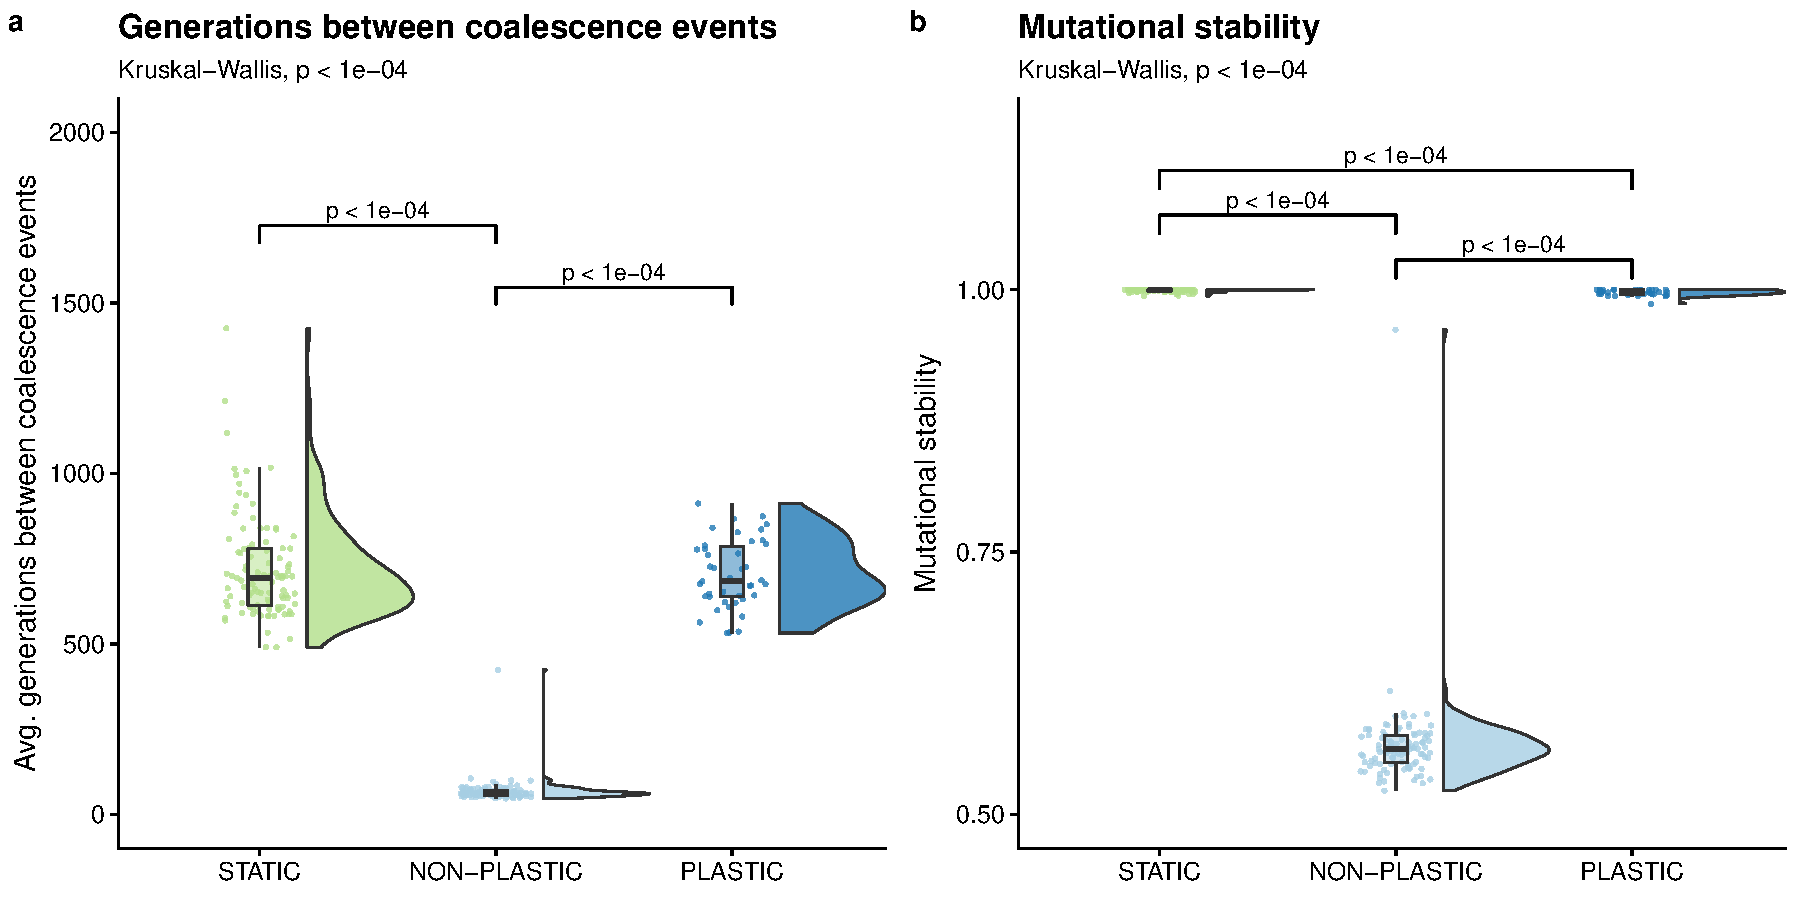
\includegraphics[width=0.66\textwidth]{chapters/03-evolutionary-consequences-of-plasticity/media/evolutionary-change-pace-panel.pdf}
    \caption{\small
    \textbf{Pace of evolutionary change.}
    Raincloud plots of 
    (a) average number of generations between coalescence events,
    and (b) mutational stability (Table \ref{chapter:consequences-of-plasticity:tab:metrics-definitions}).
    Each plot is annotated with statistically significant comparisons (Bonferroni-corrected pairwise Wilcoxon rank-sum tests).
    }
    \label{chapter:consequences-of-plasticity:fig:evolutionary-dynamics-rate}
\end{figure}

% -- Rate of evolutionary change => findings --
On average, significantly fewer generations elapsed between coalescence events in NON-PLASTIC populations than in either PLASTIC or STATIC populations (Figure \ref{chapter:consequences-of-plasticity:fig:evolutionary-dynamics-rate}a).
We also found that both STATIC and PLASTIC lineages exhibited higher mutational stability relative to that of NON-PLASTIC lineages (Figure \ref{chapter:consequences-of-plasticity:fig:evolutionary-dynamics-rate}b); that is, mutations more often caused phenotypic changes along NON-PLASTIC lineages. 
Overall, our results indicate that NON-PLASTIC populations underwent more rapid (and thus a greater amount of) evolutionary change than either PLASTIC or STATIC populations. 

% -- Mutational stability in static and plastic lineages --
While both STATIC and PLASTIC lineages exhibited high mutational stability, we found that STATIC lineages exhibited higher mutational stability than PLASTIC lineages (Figure \ref{chapter:consequences-of-plasticity:fig:evolutionary-dynamics-rate}b). 
Overall, there were rare instances of mutations that caused a change in phenotypic profile across all PLASTIC lineages.
Of these mutations, we found that over 80\% (83 out of 102) of changes to phenotypic profiles were cryptic. 
That is, the mutations affected traits that would not have been expressed in the environment that the organism was born into, but would have been expressed had the environment changed.

\begin{figure}[ht!]
    \centering
    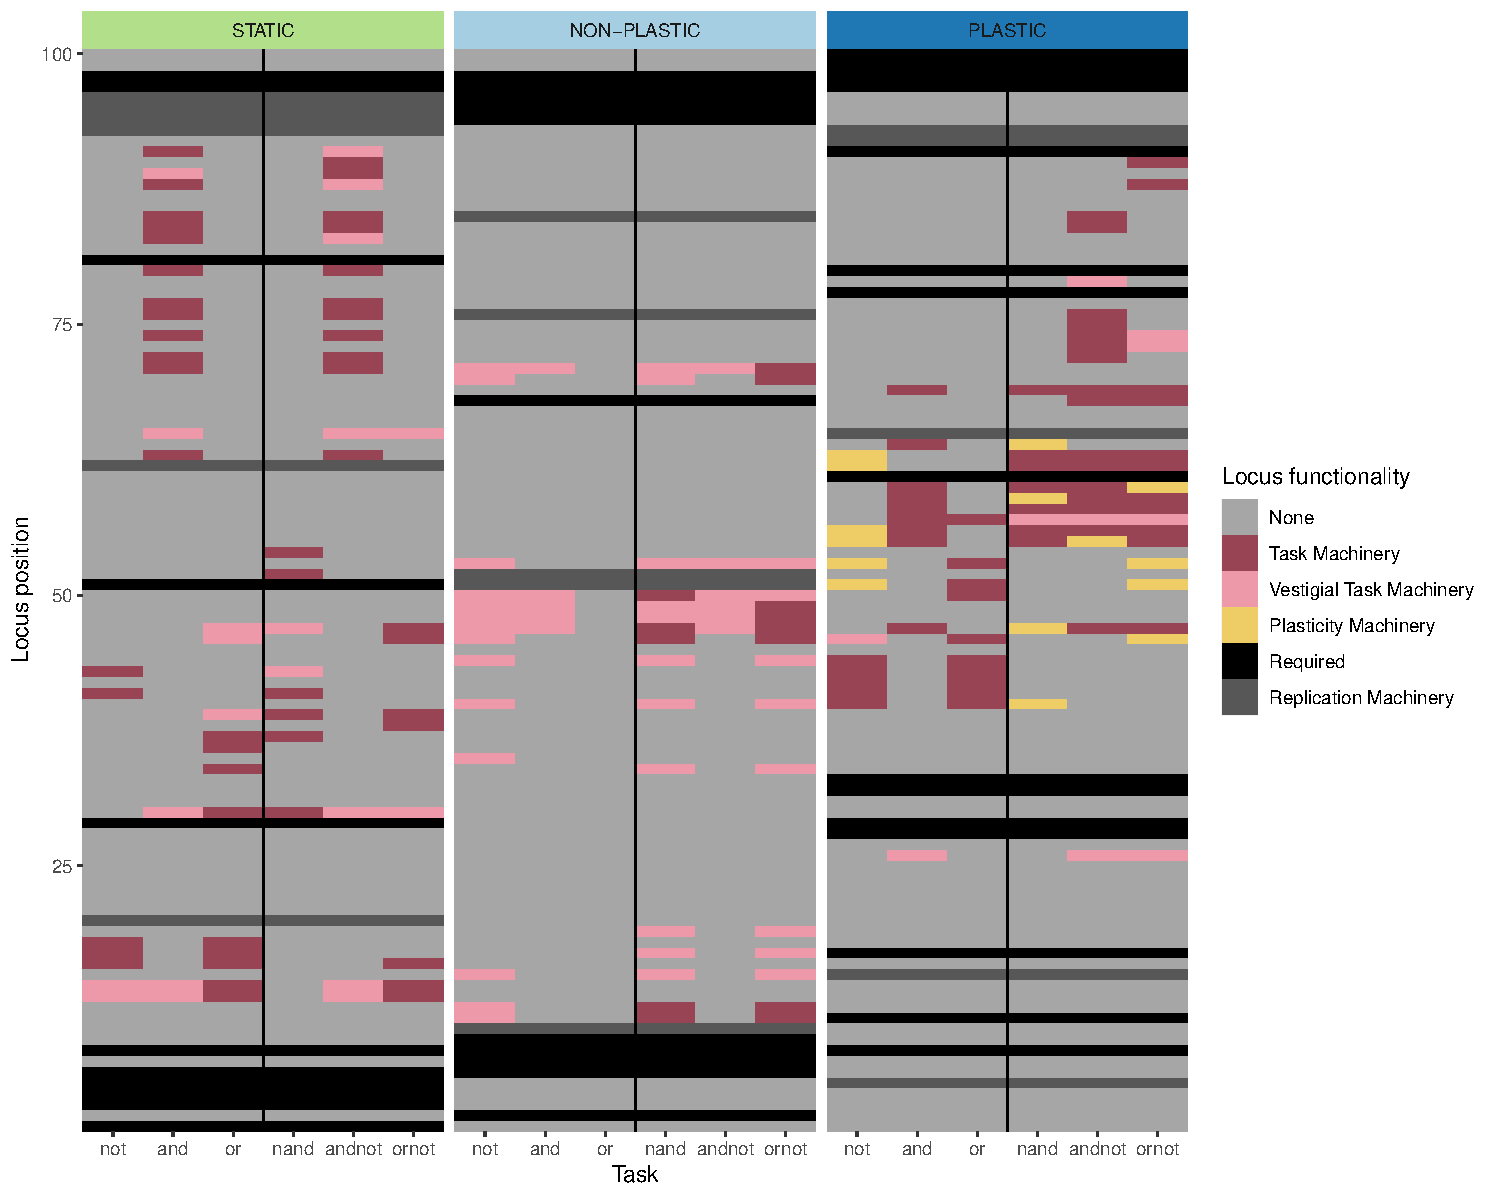
\includegraphics[width=1\textwidth]{chapters/03-evolutionary-consequences-of-plasticity/media/locus-slice-combined-color-facets.pdf}
    \caption{\small
    \textbf{Representative genetic architectures from each treatment.}
    Each box shows a representative genome from each condition at the end of Phase 2A. 
    The y-axis indicates each site in each genome, and colors indicate the function of each locus with respect to a particular task (given by the x-axis). 
    % Each of the six base tasks are shown on the x axis. 
    The vertical black line splits tasks rewarded in ENV-A (left of the line) from those rewarded in ENV-B.
    Loci colored as ``Task Machinery'' are actively involved in the performance of that task, while ``Vestigial Task Machinery'' represents loci that have not mutated, but no longer code for the task (\textit{i.e.}, a change elsewhere in the genome has disabled or modified the task). 
    ``Plasticity Machinery'' refers to loci that regulate the given task. 
    Knocking out a ``Replication Machinery'' locus negatively affects replication time, while knocking out a ``Required'' locus results in a non-viable organism. 
    }
    \label{chapter:consequences-of-plasticity:fig:architecture-locus-functionality}
\end{figure}
\begin{figure}[ht!]
    \centering
    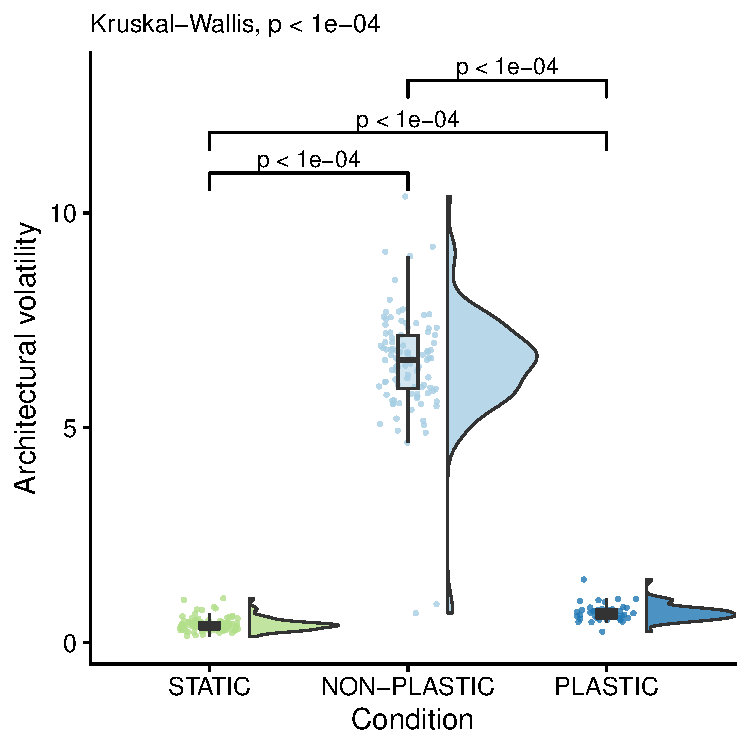
\includegraphics[width=0.35\textwidth]{chapters/03-evolutionary-consequences-of-plasticity/media/architectural-volatility.pdf}
    \caption{\small
        \textbf{Architectural volatility.}
        Raincloud plot of architecture stability (Table \ref{chapter:consequences-of-plasticity:tab:metrics-definitions}).
        The plot is annotated with statistically significant comparisons (Bonferroni-corrected pairwise Wilcoxon rank-sum tests). 
    }
    \label{chapter:consequences-of-plasticity:fig:architecture-volatility}
\end{figure}

% -- genetic architectures --
Next, we performed knockout experiments to investigate how genetic architectures evolved under the three treatment regimes. 
Thus far, we have shown that adaptive plasticity slows evolutionary change in fluctuating environments, 
but we have not determined if adaptive plasticity also alters how genetic architectures (\textit{i.e.}, how functions are arranged on genomes) change over time. 
Figure \ref{chapter:consequences-of-plasticity:fig:architecture-locus-functionality} shows the function of each locus in a representative genome from each treatment at the end of the experiment, which is also 100 updates after the environment changed from ENV-A to ENV-B in the PLASTIC and NON-PLASTIC treatments. 
The PLASTIC and STATIC genomes are capable of performing tasks from both environments, while the NON-PLASTIC genome only performs tasks rewarded in ENV-B.
We expect instructions associated with ENV-A tasks to be lost in NON-PLASTIC populations during evolution in ENV-B. 
Indeed, we assign a metabolic cost for performing ENV-A tasks in ENV-B, resulting in negative selection on performing ENV-A tasks.
Unused ENV-A tasks should also decay with evolution in ENV-B even without the metabolic cost we impose, as the associated instructions are more likely to accumulate mutations under relaxed selection \citep{lahti_relaxed_2009}.  
Alternatively, previous work in Avida has shown that tasks punished in one environment can be maintained in the genome as vestigial loci \citep{canino-koning_evolution_2016,canino-koning_fluctuating_2019} where their function is retained and co-opted for use in an alternate environment. 
Under this scenario we might expect the NON-PLASTIC genomes to retain the instructions needed for ENV-A tasks during their evolution in ENV-B.
Consistent with \cite{canino-koning_evolution_2016,canino-koning_fluctuating_2019}'s work, the NON-PLASTIC genome that we analyzed from ENV-B (Figure \ref{chapter:consequences-of-plasticity:fig:architecture-locus-functionality}) contains substantial vestigial loci for ENV-A's NOT task; we also found that these vestigial sites were exapted for ENV-B's NAND and OR-NOT tasks. 
Indeed, visual inspection of locus functions over entire lineages shows that NON-PLASTIC lineages often contain loci that are continuously cycling between coding for ENV-A tasks and ENV-B tasks.
Further, NON-PLASTIC lineages exhibited significantly higher architectural volatility than STATIC or PLASTIC lineages (Figure~\ref{chapter:consequences-of-plasticity:fig:architecture-volatility}).

% -- in general, PLASTIC and STATIC more similar than NON-PLASTIC --
In general, the evolution of adaptive plasticity stabilized PLASTIC treatment populations against environmental fluctuations, and their evolutionary dynamics more closely resembled those of populations evolving in a static environment.
We observed no significant difference in the number and frequency of coalescence events in PLASTIC and STATIC populations.
We did, however, observe small, but statistically significant, differences in each of the following metrics: elapsed generations, mutation counts, mutational stability, and architectural volatility between PLASTIC and STATIC populations (see supplemental material \citealt{consequences_of_plasticity_supplemental_material_2021}).

\subsection{Adaptively plastic populations retain more novel tasks than non-plastic populations in fluctuating environments}

%%%%%%%%%%%%%%%%%%%%%%%%%%%%%%%%%
% Results to report (2021-01-31)
% - Number of plastic replicates
% - Final dominant genotype # novel traits
%   - non-plastic < (plastic == static)
% - Final population (1% threshold): 
%   - non-plastic < plastic < static
% - Final population (1% threshold) discovered:
%   - non-plastic > (plastic ~~ static)
% - Lineage tasks discovered
%   - non-plastic > static ~>(nosig) plastic
% - Lineage tasks discovered / step
%   - (static ~~ plastic) > non-plastic 
% - Lineage tasks lost
%   - non-plastic > static > plastic
% - Lineage tasks lost / step
%   - non-plastic > static > plastic

% - tasks discovered per generation(?)
%   - NON-PLASTIC [0.00014358046266055] ~~ STATIC [0.00015363220504867] > PLASTIC [0.000117695011124939]
% - tasks lost per generation(?)
%   - NON-PLASTIC [0.0022026054610079] > STATIC [0.000161396283669756] > PLASTIC [6.25141973661864e-05]
%%%%%%%%%%%%%%%%%%%%%%%%%%%%%%%%%

\begin{figure}[ht!]
    \centering
    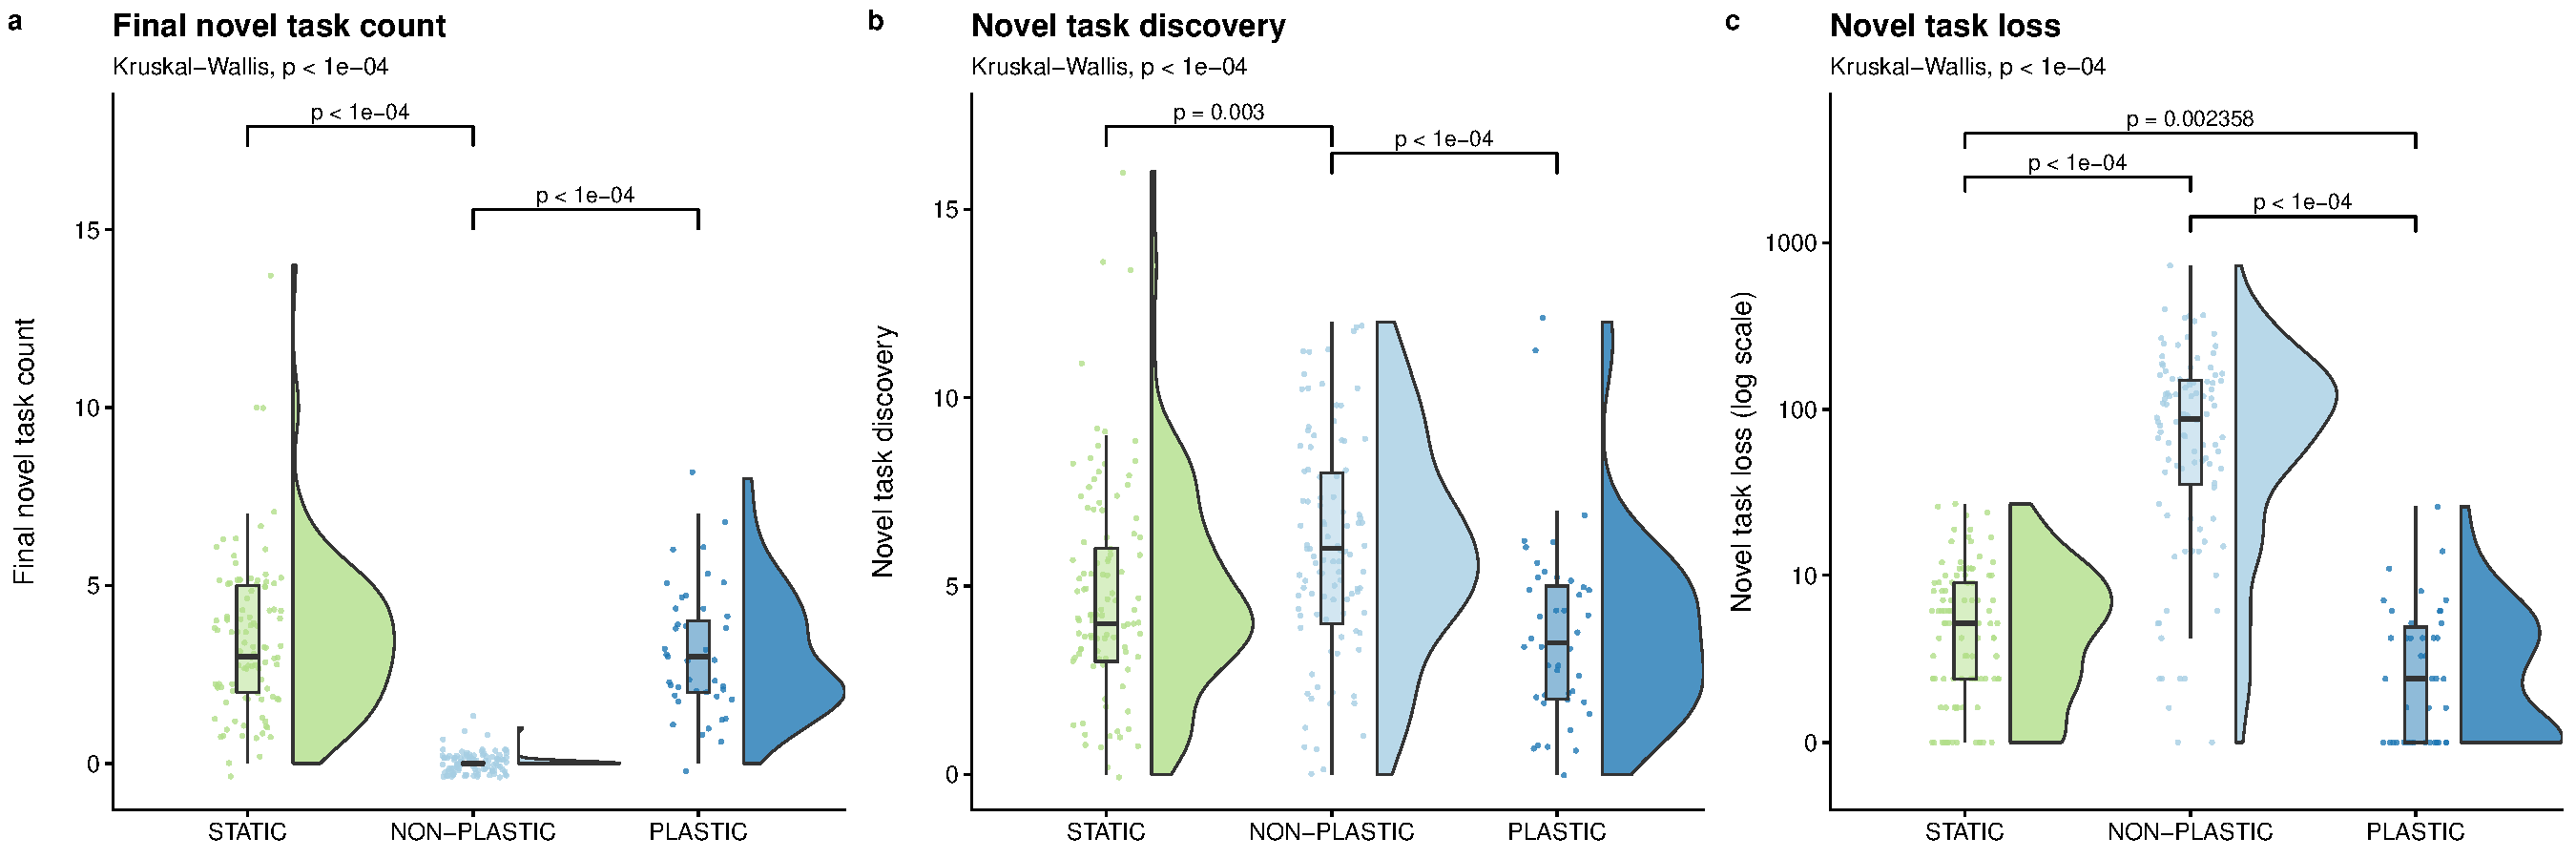
\includegraphics[width=\textwidth]{chapters/03-evolutionary-consequences-of-plasticity/media/complex-traits-magnitude-panel.pdf}
    \caption{\small
    \textbf{Novel task evolution.}
    Raincloud plots of 
    (a) final novel task count,
    (b) novel task discovery,
    and (c) novel task loss.
    See Table \ref{chapter:consequences-of-plasticity:tab:metrics-definitions} for descriptions of each metric.
    Each plot is annotated with statistically significant comparisons (Bonferroni-corrected pairwise Wilcoxon rank-sum tests).
    Note that adaptive phenotypic plasticity evolved in \novelTraitsPlasticReps\ of \novelTraitsReplicates\ replicates from the PLASTIC treatment during phase one of this experiment; 
    we used this more limited group to found \novelTraitsPlasticReps\ phase-two PLASTIC replicates from which we report these PLASTIC data.
    }
    \label{chapter:consequences-of-plasticity:fig:complex-traits-magnitude}
\end{figure}

% -- What did we test? --
We have so far shown that adaptive plasticity constrains the rate of evolutionary change in fluctuating environments.
However, it is unclear how this dynamic influences the evolution of novel tasks.
Based on their relative rates of evolutionary change, we might expect NON-PLASTIC-treatment populations to evolve more novel tasks than PLASTIC-treatment populations.
But, how much of the evolutionary change in NON-PLASTIC populations is useful for exploring novel regions of the fitness landscape versus continually rediscovering the same regions?

% - Magnitude of exploration/exploitation -
To answer this question, we quantified the number of novel tasks performed by a representative organism in the final population of each replicate.
We found that both PLASTIC and STATIC populations had significantly higher final task counts than NON-PLASTIC populations at the end of the experiment (Figure~\ref{chapter:consequences-of-plasticity:fig:complex-traits-magnitude}a). 
The final novel task count in PLASTIC and STATIC lineages could be higher than that of the NON-PLASTIC lineages for several non-mutually exclusive reasons. 
One possibility is that PLASTIC and STATIC lineages could be exploring a larger area of the fitness landscape when compared to NON-PLASTIC lineages. 
Another possibility is that the propensity of the NON-PLASTIC lineages to maintain novel traits could be significantly lower than PLASTIC and STATIC lineages. 
When we looked at the total sum of novel tasks discovered by each of the PLASTIC, STATIC, and NON-PLASTIC lineages, we found that the NON-PLASTIC lineages explored a significantly larger area of the fitness landscape (Figure~\ref{chapter:consequences-of-plasticity:fig:complex-traits-magnitude}b).
Although the NON-PLASTIC lineages discovered more novel tasks, those lineages also exhibited significantly higher novel task loss when compared to PLASTIC and STATIC lineages (Figure~\ref{chapter:consequences-of-plasticity:fig:complex-traits-magnitude}c). 

\begin{figure}[ht!]
    \centering
    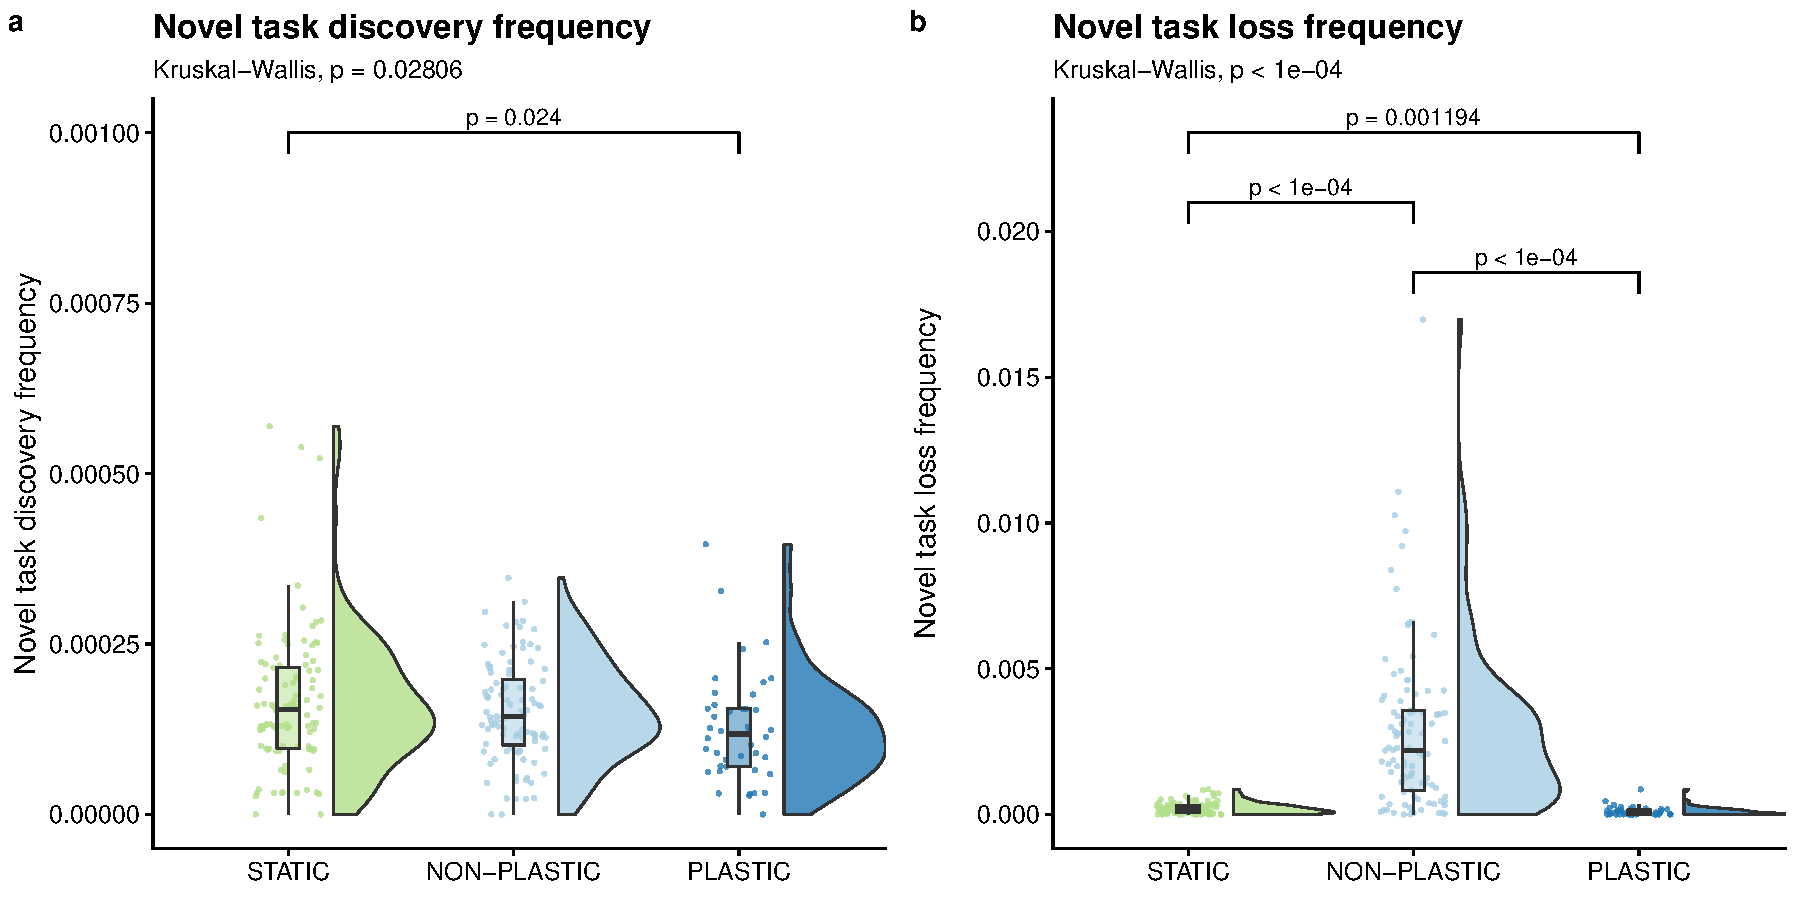
\includegraphics[width=0.66\textwidth]{chapters/03-evolutionary-consequences-of-plasticity/media/complex-traits-pace-panel.pdf}
    \caption{\small
    \textbf{Rates of novel task evolution.}
    Raincloud plots of 
    (a) novel task discovery frequency
    and (b) novel task loss frequency.
    Each plot is annotated with statistically significant comparisons (Bonferroni-corrected pairwise Wilcoxon rank-sum tests).
    }
    \label{chapter:consequences-of-plasticity:fig:complex-traits-rate}
\end{figure}

% - Rates of exploration/exploitation -
A larger number of generations elapsed in NON-PLASTIC populations than in PLASTIC or STATIC populations during our experiment \citep{consequences_of_plasticity_supplemental_material_2021}.
Are NON-PLASTIC lineages discovering and losing novel tasks more frequently than PLASTIC or STATIC lineages, or are our observations a result of differences in generational turnover?
To answer this question, we converted the metrics of novel task discovery and novel task loss to rates by dividing each metric by the number of elapsed generations along the associated representative lineages.
We found no significant difference in the frequency of novel task discovery between NON-PLASTIC and STATIC lineages, and we found that PLASTIC lineages had a lower frequency of novel task discovery than STATIC lineages (Figure~\ref{chapter:consequences-of-plasticity:fig:complex-traits-rate}a).
Therefore, we cannot reject the possibility that the larger magnitude of task discovery in NON-PLASTIC lineages was driven by a larger number of elapsed generations.
NON-PLASTIC lineages had a higher frequency of task loss than either PLASTIC or STATIC lineages, and PLASTIC lineages tended to have a lower frequency of novel task loss than STATIC lineages (Figure~\ref{chapter:consequences-of-plasticity:fig:complex-traits-rate}b). 

% - Characterizing trait loss -
Next, we examined the frequency at which novel task loss along lineages co-occurred with the loss or gain of any of the six base tasks.
Across all NON-PLASTIC representative lineages, over 97\% (10998 out of 11229) of instances of novel task loss co-occurred with a simultaneous change in base task profile.
In contrast, across all PLASTIC and STATIC dominant lineages, we observed that approximately 20\% (29 out of 142) and 2\% (13 out of 631), respectively, of instances of novel task loss co-occurred with a simultaneous change in base task profile.
As such, the losses of novel tasks in NON-PLASTIC lineages appear to be primarily due to hitchhiking.

\begin{raggedright}
\subsection{Lineages without plasticity that evolve in fluctuating environments express more deleterious tasks}
\end{raggedright}

%%%%%%
% 2021-02-05 - Results
% - Number of offspring on lineage where hitchhiker instruction execution increases (i.e., instances of hitchhiking)
%   - PLASTIC ~~ STATIC < NON-PLASTIC
% - Hitchhiker instruction increases / offspring on lineage
%   - PLASTIC ~~ STATIC < NON-PLASTIC
% - What fraction of mutations that increase hitchhiker instruction execution co-occur with base trait changes?
%   - NON-PLASTIC > PLASTIC ~~ STATIC
% - What about unexpressed vs expressed trait changes in plastic populations? (plastic only)
%   - Not much hitchhiking. Did not find evidence that hitchiking occurring as cryptic variation in unexpressed phenotype.
%%%%%%

Phenotypic plasticity allows for genetic variation to accumulate in genomic regions that are unexpressed, which could lead to the fixation of deleterious instructions in PLASTIC populations.
However, in NON-PLASTIC lineages we observe a higher rate of novel task loss, indicating that they may be more susceptible to deleterious mutations (Figure \ref{chapter:consequences-of-plasticity:fig:complex-traits-rate}).

Therefore, in experiment phase 2C, we tested whether adaptive phenotypic plasticity can increase the incidence of deleterious task performance. 
Specifically, we added an instruction that triggered a ``poisonous'' task and measured the number of times it was executed.
Each execution of the  \code{poison} instruction reduces an organism's fitness by 10\%. 
At the beginning of phase 2C, the \code{poison} instruction is not present in the population, as it was not part of the instruction set during phase one of evolution.
Accordingly, if a \code{poison} instruction fixes in a population, it must be the result of evolutionary dynamics during phase 2C, including cryptic variation or hitchhiking. 

\begin{figure}[ht!]
    \centering
    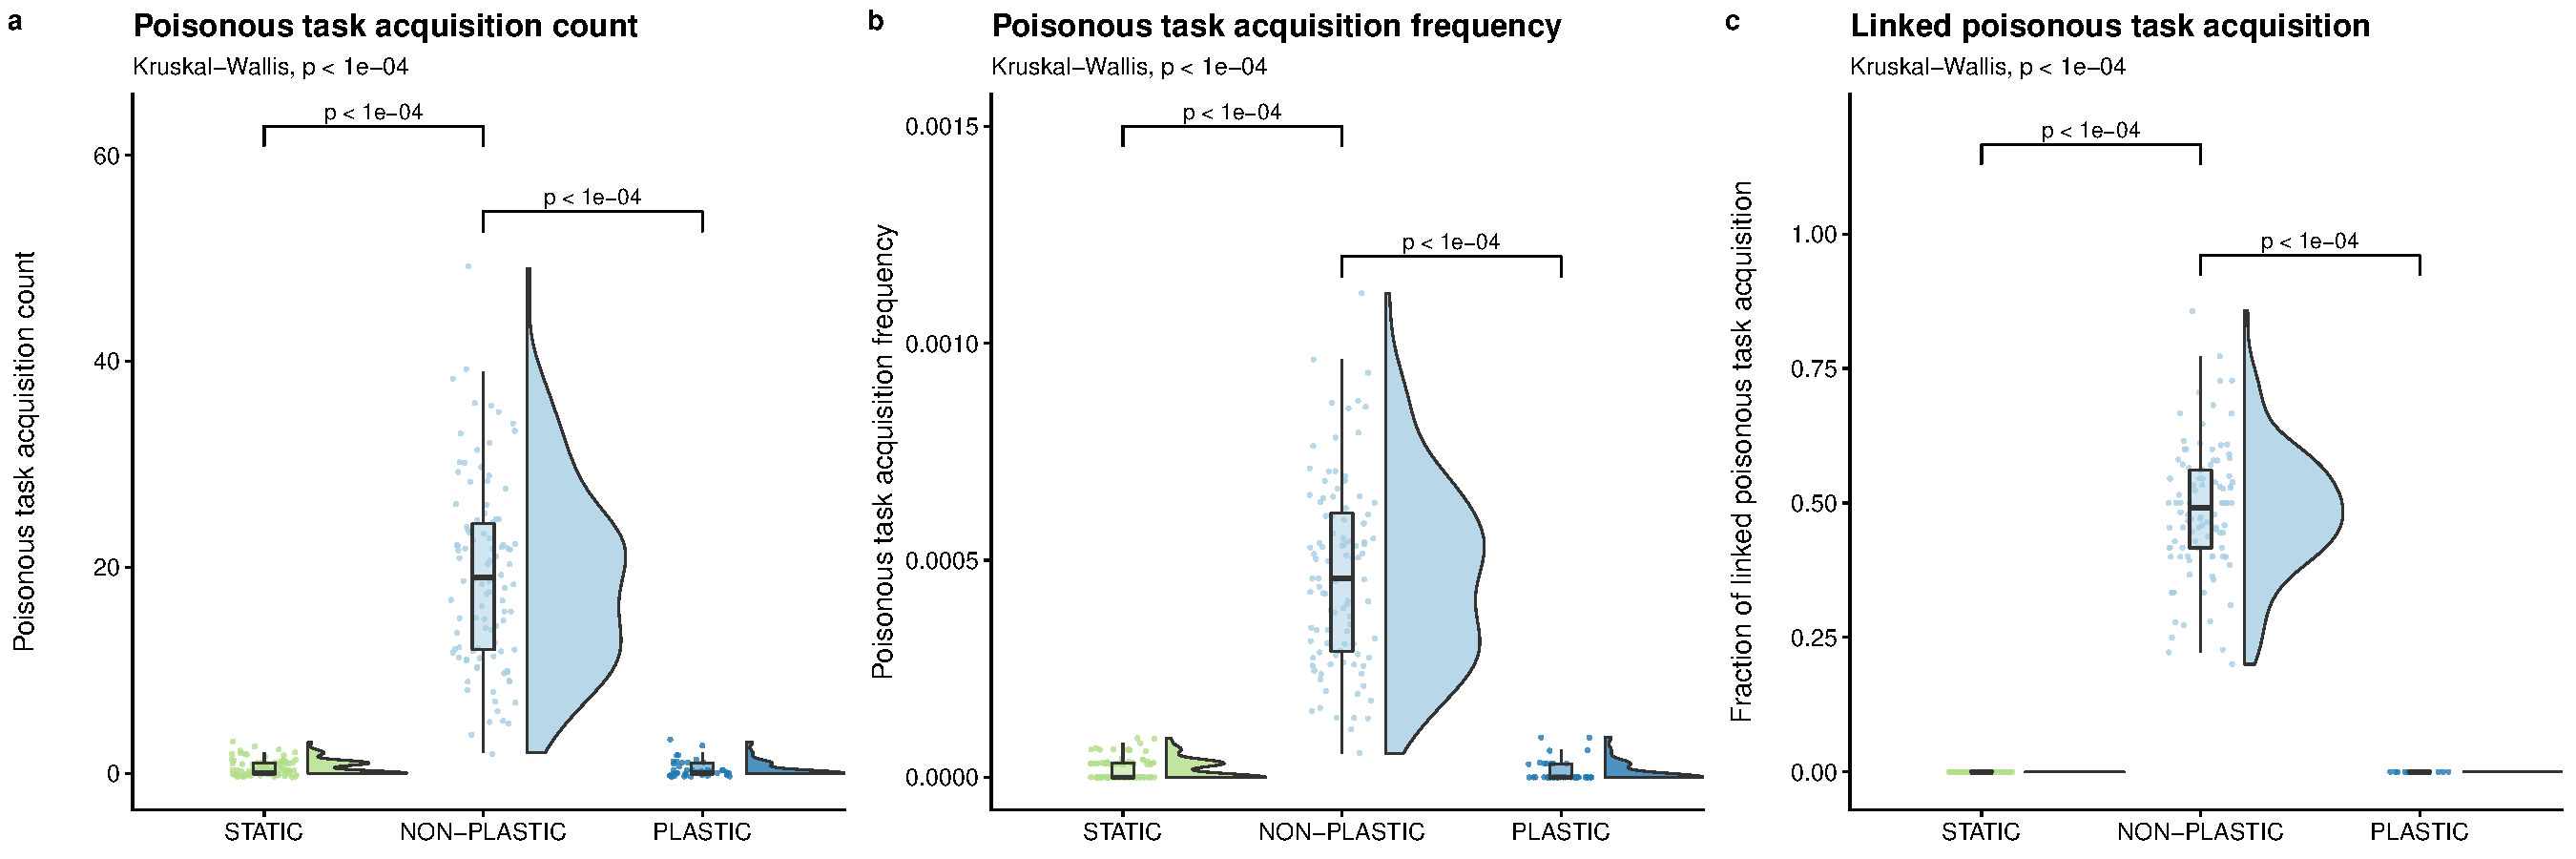
\includegraphics[width=1.0\textwidth]{chapters/03-evolutionary-consequences-of-plasticity/media/poison-accumulation-panel.pdf}
    \caption{\small
    \textbf{Deleterious instruction accumulation.}
    Raincloud plots of 
    (a) poisonous task acquisition,
    (b) poisonous task acquisition frequency,
    and (c) the proportion of mutations that increase poisonous task performance along a lineage that co-occur with a change in phenotypic profile.
    Each plot is annotated with statistically significant comparisons (Bonferroni-corrected pairwise Wilcoxon rank-sum tests).
    Note that adaptive phenotypic plasticity evolved in \deleteriousHitchhikingPlasticReps\ of \deleteriousHitchhikingReplicates\ replicates from the PLASTIC treatment during phase one of this experiment; 
    we used this more limited group to found \deleteriousHitchhikingPlasticReps\ phase-two PLASTIC replicates from which we report these PLASTIC data.
    }
    \label{chapter:consequences-of-plasticity:fig:deleterious-hitchhiking}
\end{figure}

% -- Instruction execution by final dominant & along lineage --
\vspace{\baselineskip}
At the end of our experiment, no representative organisms from the PLASTIC or STATIC treatments performed the poisonous task under any environmental condition; however, representative organisms in 14\% of replicates of the NON-PLASTIC treatment performed the poisonous task at least once. 
NON-PLASTIC lineages contained significantly more mutations that conferred the poisonous task as compared to PLASTIC or STATIC lineages (Figure \ref{chapter:consequences-of-plasticity:fig:deleterious-hitchhiking}a).
This result does not change when we normalize by the number of generations represented in the given lineage (Figure \ref{chapter:consequences-of-plasticity:fig:deleterious-hitchhiking}b).

% -- When/where does hitchhiking take place? --
Next, we measured how often mutations that increased poisonous task performance co-occurred with changes to the base task profile within representative lineages.
A poisonous instruction can fix in a lineage by having a beneficial effect that outweighs its inherent cost (\textit{e.g.}, knocking out a punished task) or through linkage with a secondary beneficial mutation at another site within in the genome.
Across all NON-PLASTIC representative lineages, we found that approximately 49\% (956 out of 1916) of mutations that increased poisonous task expression co-occurred with a change in the base task profile (Figure \ref{chapter:consequences-of-plasticity:fig:deleterious-hitchhiking}c).
In all representative lineages from the PLASTIC treatment, only 18 mutations increased poisonous task expression, and none co-occurred with a change in base task profile (Figure \ref{chapter:consequences-of-plasticity:fig:deleterious-hitchhiking}c).
Likewise, only 58 mutations increased poisonous task performance in all representative lineages from the STATIC treatment, and none co-occurred with a change in base task profile (Figure \ref{chapter:consequences-of-plasticity:fig:deleterious-hitchhiking}c).
We did not find compelling evidence that the few mutations that conferred poisonous task expression in PLASTIC lineages occurred as cryptic variation.

We repeated this experiment with 3\% and 30\% metabolic rate penalties associated with the poisonous task, which produced results that were consistent with those reported here \citep{consequences_of_plasticity_supplemental_material_2021}.